\subsection{Music recommendation}
Collaborative filtering is the part of recommender systems that predicts users' preferences for particular items. The major challenge in predicting users' listening counts, as in our task, is that the available user-artist entries are usually too few and sometimes a method's performance relies on a good initial estimation of the unknown entries. 
We therefore decided to implement besides the common KNN, Kmeans also ALS \cite{Zhou:2008}, which uses only the known listening counts and avoids dependency on initial estimations.

\subsection{Data description}
The training data consists in a matrix $Ytrain$ of $1774$ users and $15802$ artists. Entry $Ytrain(i,j)$ expresses how many times user $i$ has listened to artist $j$. An entry of 0 means we do not have information for that $(user, artist, count)$ triple. We are also given the friendship graph of the $1774$ users stored as an adjacency matrix.

\subsection{Exploratory Data Analysis}

The matrix $Ytrain$ is very sparse with a density of only $0.26\%$, corresponding to $69617$ $(user, artist, count)$ triples. The variance of the entries' values is very high, the maximum  being $352698$ and average listening count per user and per artist of $5.52$ and $5.46$ respectively. There were also $1262$ artists for which no information was provided. \par \noindent A histogram of all the listening counts tell us that the known entries follow a heavy tail distribution. The large counts represent a small number of popular items, the well-known artists, and the rest are located in the long tail. One method to transform skewed data such that it becomes more gaussian distributed is to use the Box-Cox transform which is equivalent with taking the log of the data (for  high and positive values). This transformation will make the distances between listening counts much smaller and will reduce the influence on error of the $(user,artist,count)$ triples with very large counts.
\par The results after the data transformation can be seen in Fig. \ref{fig:user_artist_distribution}. The distribution of the user counts and of the artist counts are closer to a normal distribution. We notice there are a few larger entries with values greater than 10. These will have a higher impact on the untransformed data evaluation. 

%An off by 1 error here will have more impact than on the small entries.

%\begin{figure}[h]
%  \centering
%  \begin{subfigure}[b]{0.45\textwidth}
%   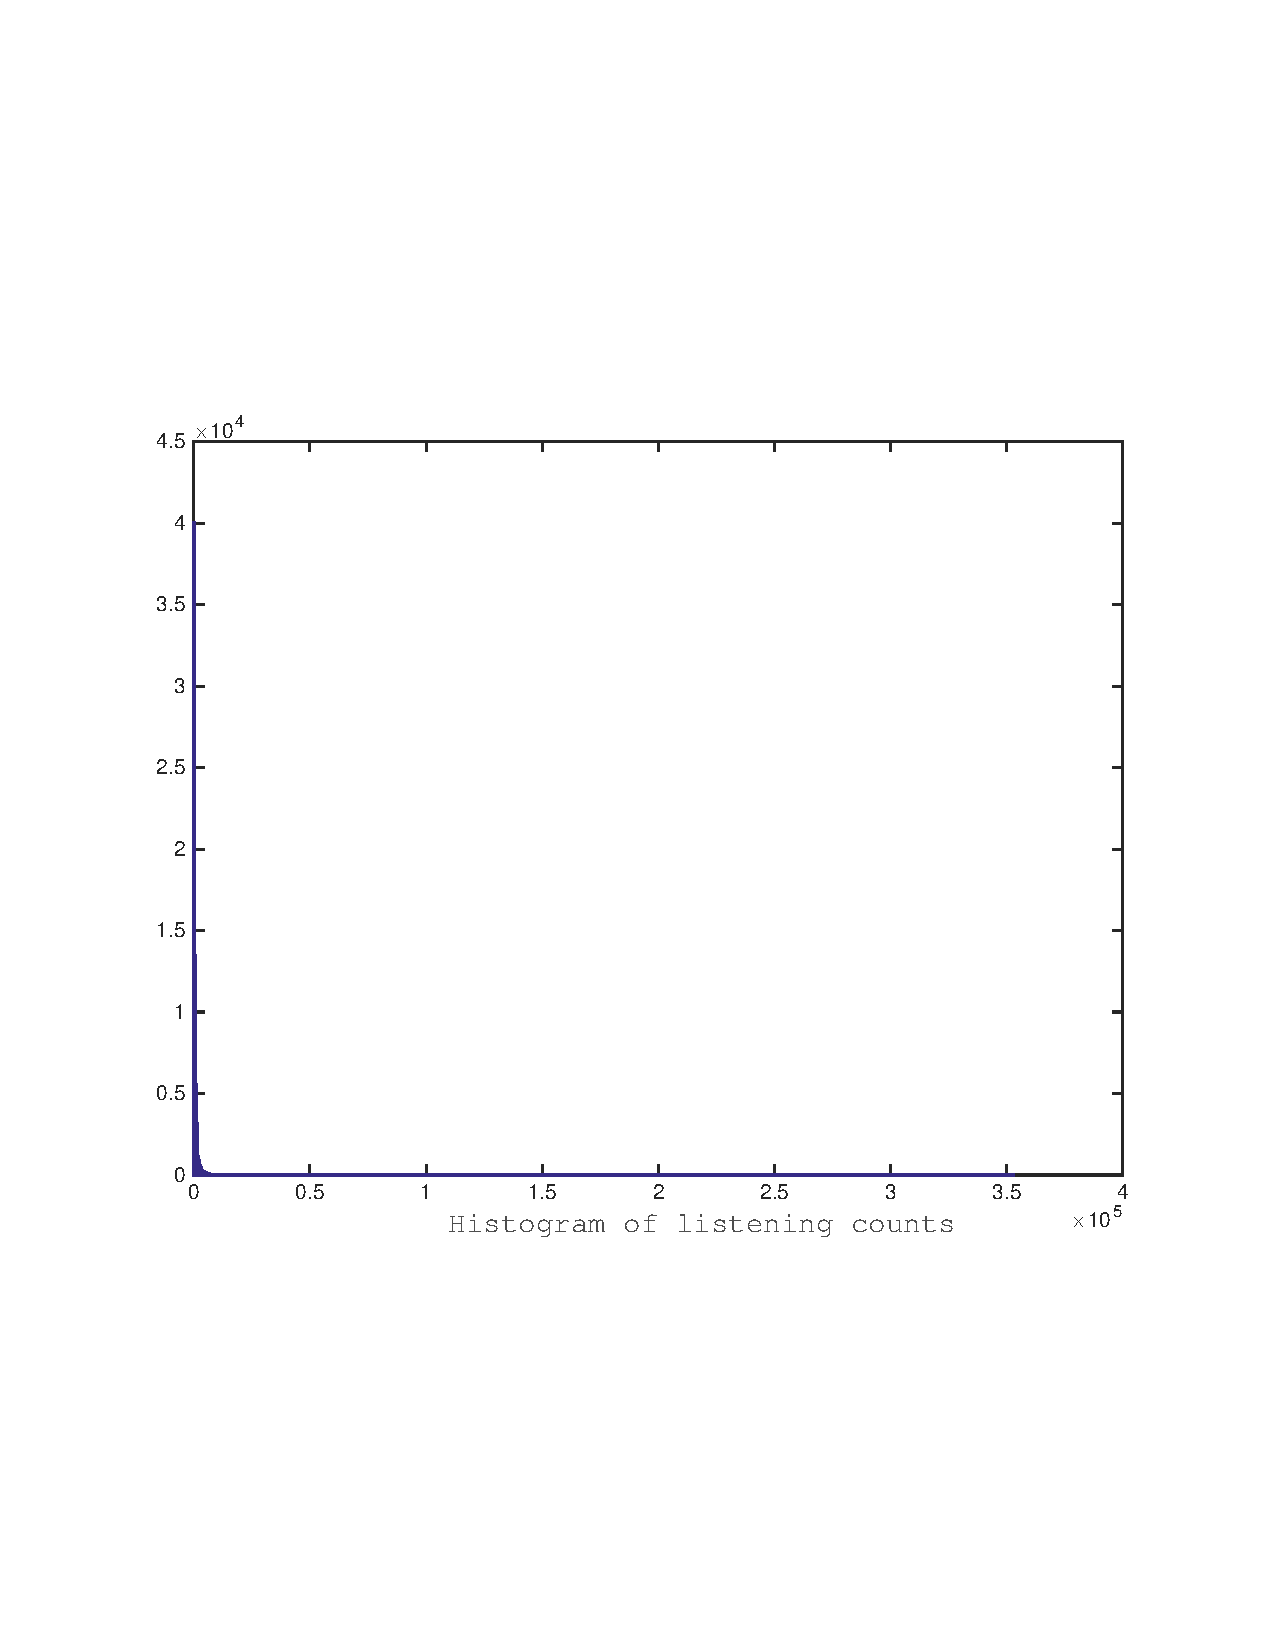
\includegraphics[width=\textwidth]{figures/histYtrain_crop.pdf}
%    \caption{Before data transformation}
%  \end{subfigure}
%  \begin{subfigure}[b]{0.45\textwidth}
 %   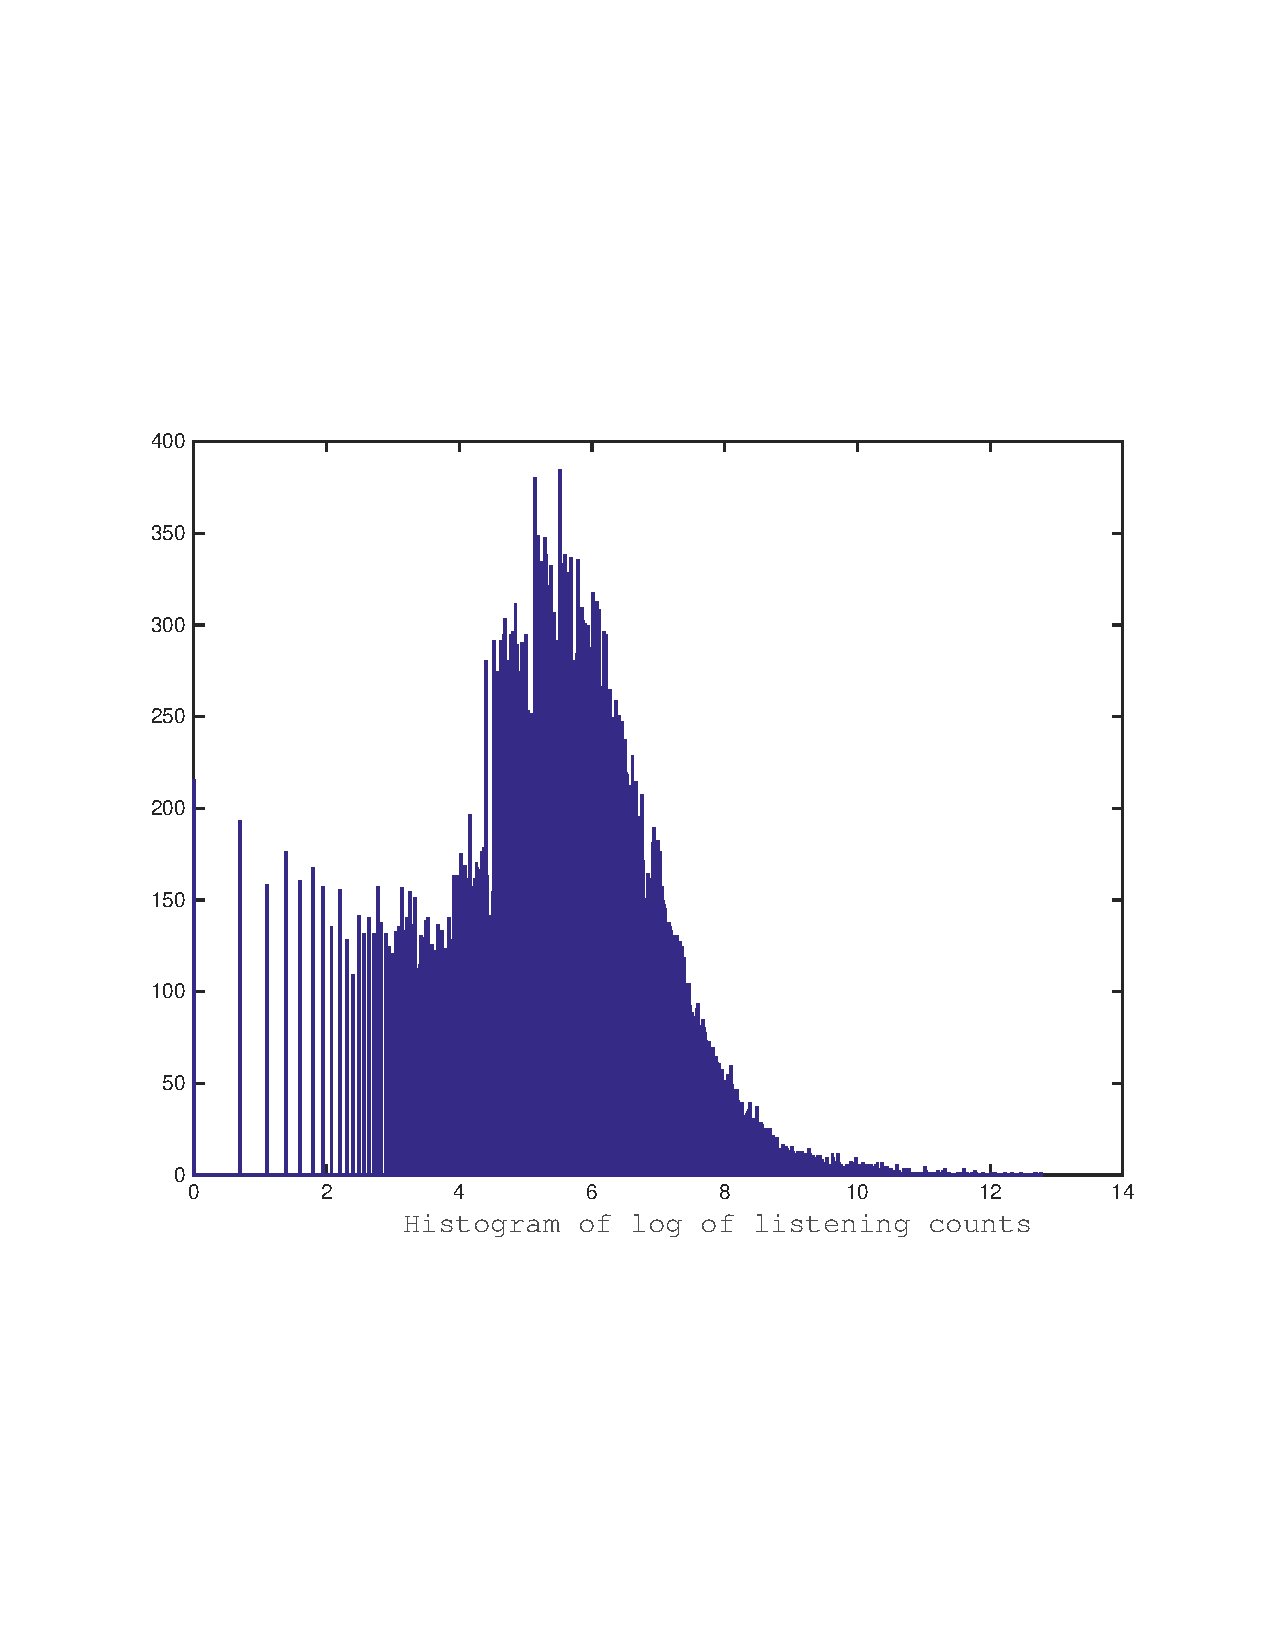
\includegraphics[width=\textwidth]{figures/histLogYtrain_crop.pdf}
 %   \caption{After data transformation}
 % \end{subfigure}
 % \caption{Distribution of all listening counts}
 % \label{fig:count_distribution}
%\end{figure}

\begin{figure}[h]
  \centering
  \begin{subfigure}[b]{0.40\textwidth}
   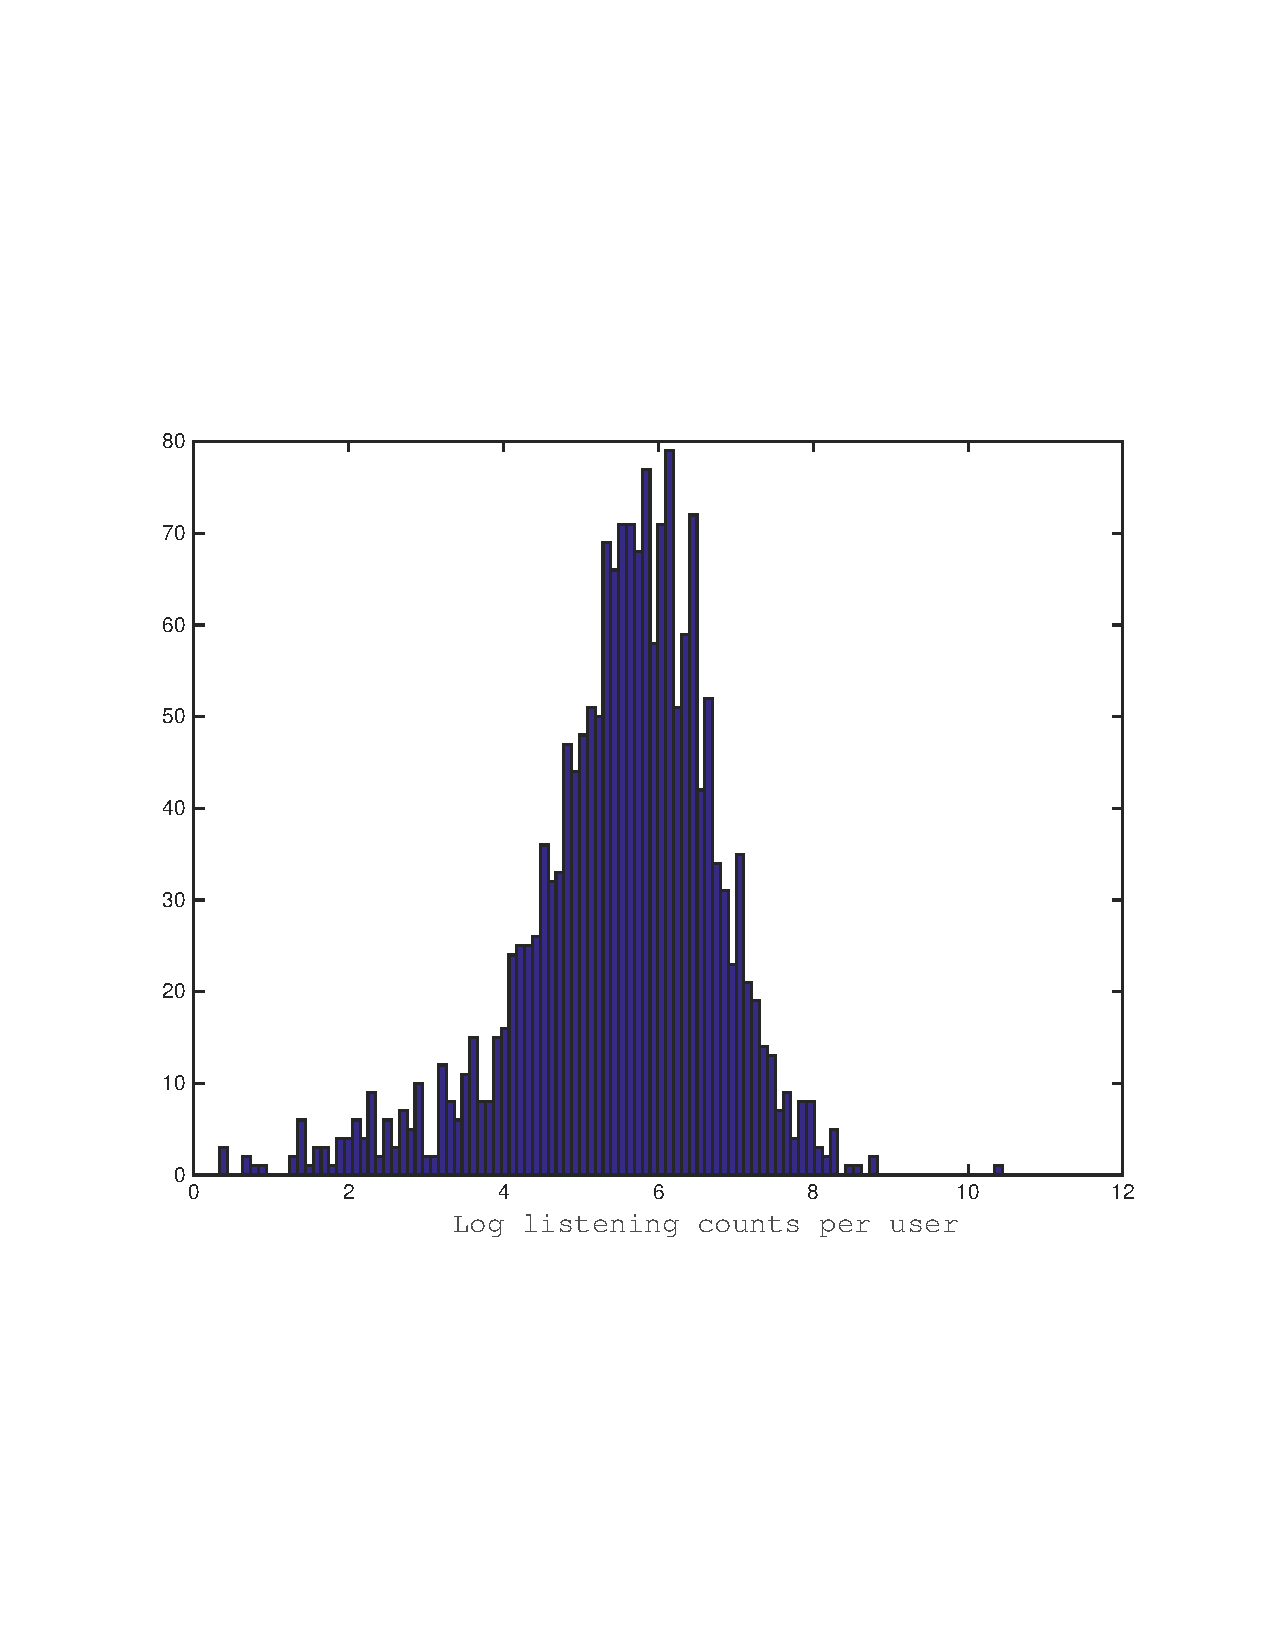
\includegraphics[width=\textwidth]{figures/histCountPerUser.pdf}
    \caption{}
  \end{subfigure}
  \begin{subfigure}[b]{0.40\textwidth}
    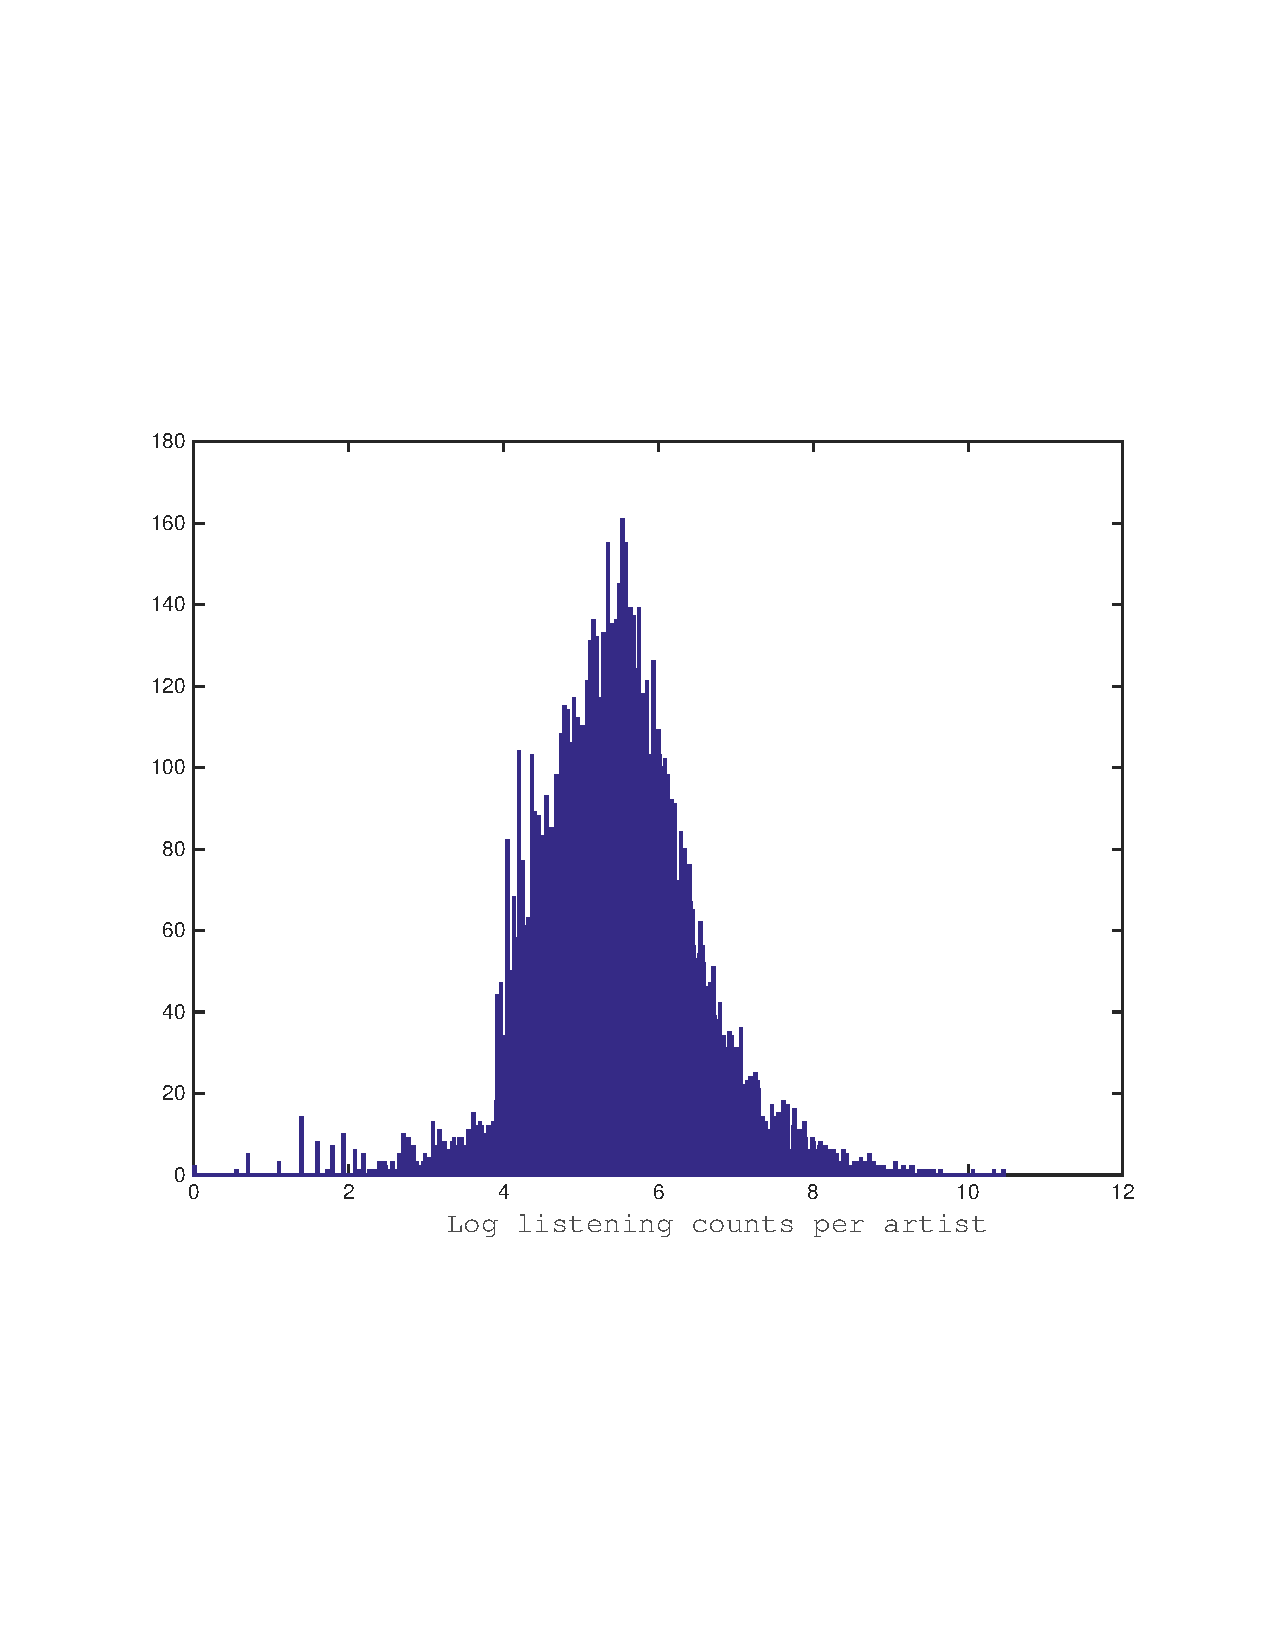
\includegraphics[width=\textwidth]{figures/histCountPerArtist.pdf}
    \caption{}
  \end{subfigure}
  \caption{Distribution of listening counts}
  \label{fig:user_artist_distribution}
\end{figure}

 
\subsection{Task 1 - Weak Prediction}
In all our experiments we used 10-fold cross validation and repeated the experiments twice. For the first task, we randomly omit 10 entries for every artist. Splitting the data was more difficult since we needed to make sure we do not remove all the entries for an artist. In the training data, if an artist has $m$ entries with $m < 10$, then we keep $m-1$ entries for testing, such that we still have at least one element for training.
 
\subsection{Baseline}
There are three simple basic predictions one can try: the global average count, the average count per user and the average count per artist prediction. These methods give following MAE results:  1.11 ($\pm$ 0.0079), 0.64 ($\pm$ 0.0042) and 1.21 ($\pm$ 0.0092). User mean average performed twice as good as the others. As it can be seen in the user mean plot (Fig. \ref{fig:MeanStdCountPerUser}), the variation of the counts per user are pretty small, less than 1 for most of the users with a few exceptions. The mean of the listening counts of an user is therefore a good estimate for a weak prediction  entry of that user.

%We note that the final MAE is composed of various values, small and large. In Fig we can see a ploto of the MAE error terms in log format.

\subsubsection{KNN}
K-nearest neighbors (KNN) algorithm is the first approach we tried for task 1. In KNN, we tried to find the most similar k users as nearest neighbors of a given user, and predict the listening count(s) of a user for a given artist. The algorithm has two important steps- calculating the similarity between users and analyzing the nearest neighbors to predict the listening count(s) of a given user. 

For measuring similarity between two users, we used the Pearson metric. We note $C(u,v)$ holds the set of artists that is common for users $u$ and $v$, and $ \bar{Y}train_u,  \bar{Y}train_v$  are average listening count for user $u$ and $v$ respectively:
\begin{equation}
  similarity(u, v)=\frac{\sum_{i\in C(u,v)} (Ytrain_{u,i} - \bar{Y}train_u)(Ytrain_{v,i} - \bar{Ytrain_v})}{\sqrt{\sum_{i\in C(u,v)} (Ytrain_{u,i} - \bar{Y}train_{u})^2} \sqrt{\sum_{i\in C(u,v)} (Ytrain_{v,i} - \bar{Y}train_{v})^2}}
\end{equation}
In recommendation phase, the following formula gives the predicted listening count of user $u$ for artist $i$:
 \begin{equation}
  p(u, i)=\frac{\sum_{k \in Neighbor(u)} similarity(u, k) (Ytrain_{k,i} - \bar{Y}train_k)}{\sum_{k \in Neighbor(u)} | similarity(u, k) |} + \bar{Y}train_u
\end{equation}
The best value for the number of nearest neighbors, $k$ depends on the data. We selected the best $k$, among $[5, 10, 15, 20, 30]$, using cross-validation technique. As can be seen from the Fig. \ref{fig:KNN_kvalues}, increasing the $k$ value up to $10$ reduces both test and train error. After $10$, further increasing the value of $k$ doesn't change the test error much but continues to reduce the train error for our data. From the cross validation result, we found the optimal number of nearest neighbors to be 15.

\begin{figure}[h]
\begin{minipage}{\textwidth}
  \begin{minipage}[b]{0.45\textwidth}
    \centering
    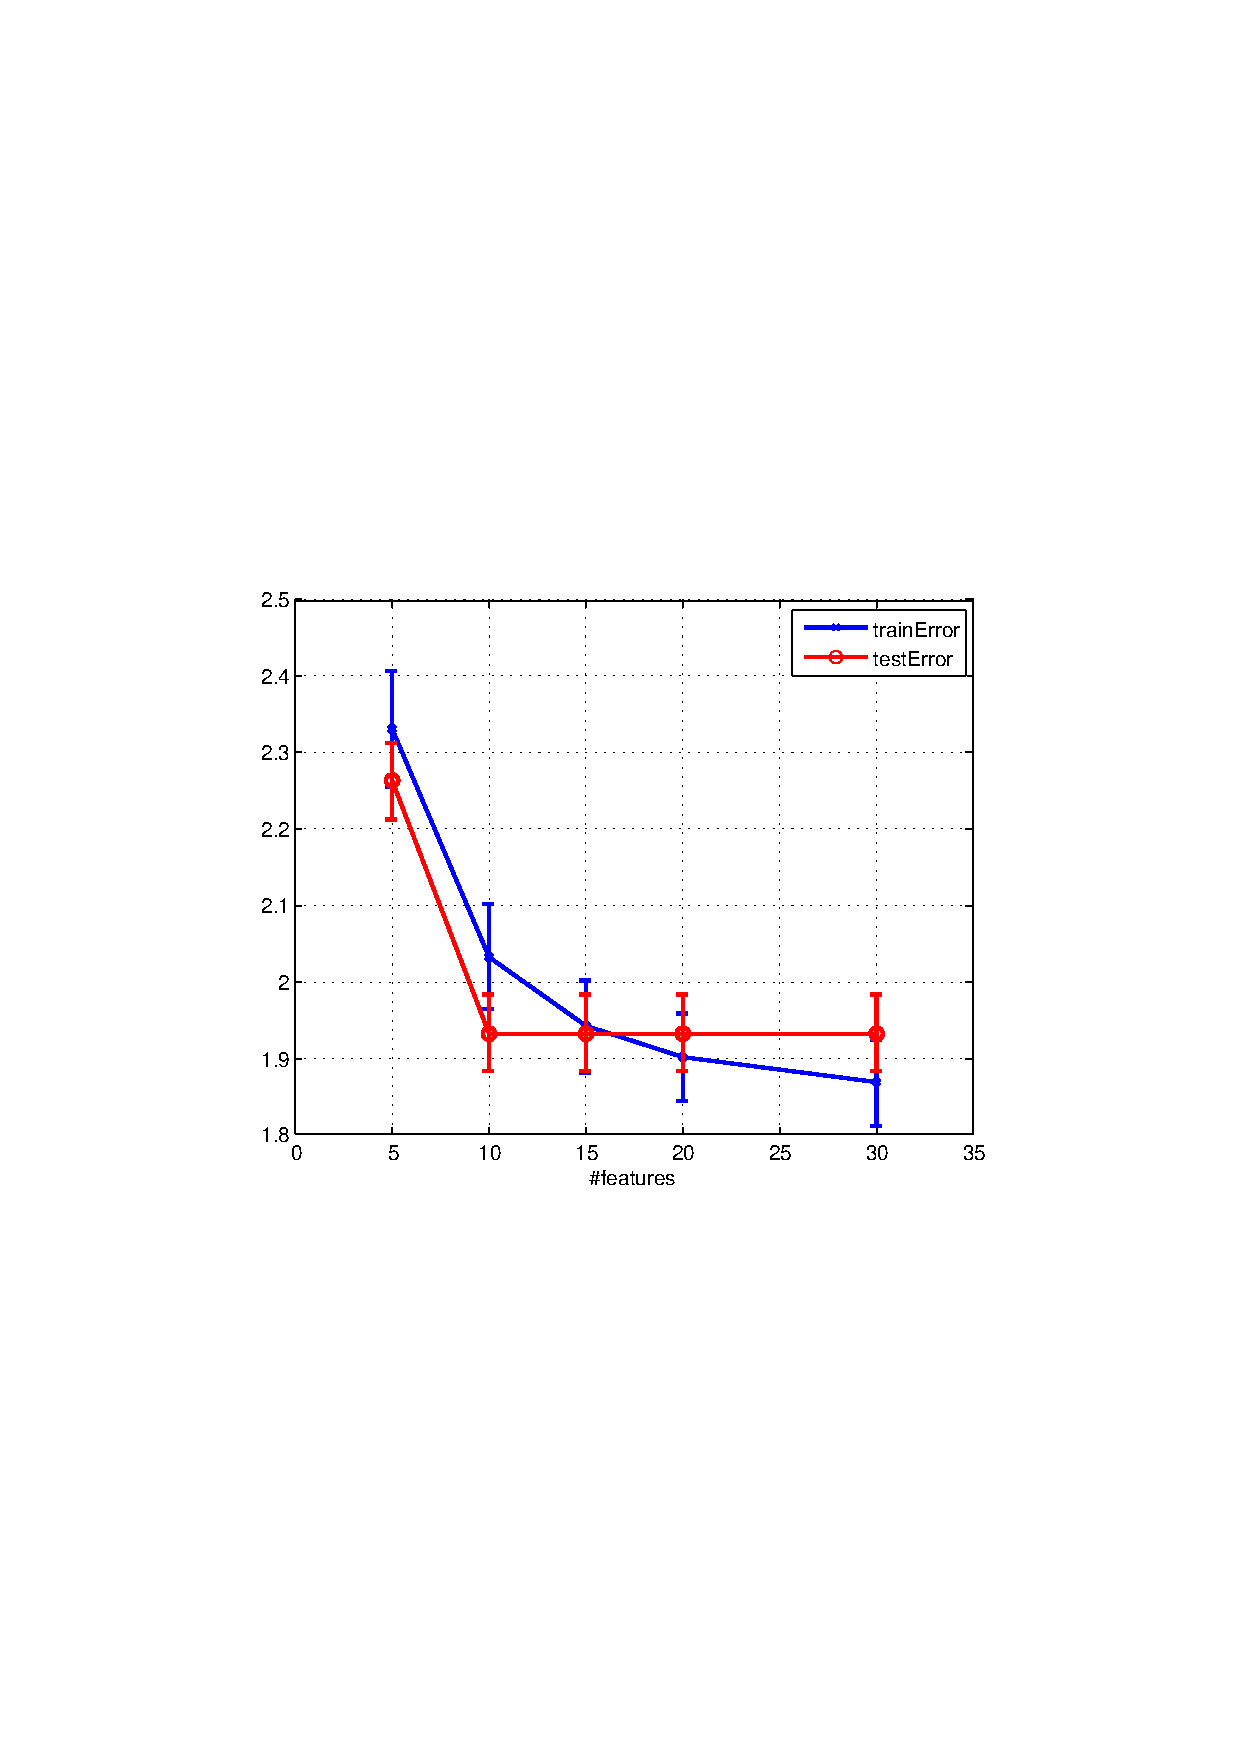
\includegraphics[clip, trim=4cm 9.2cm 3.5cm 9cm, width=\textwidth]{figures/KNN_kvalue.pdf}
    %\captionof{figure}{Comparison of Train and Test errors with different k values}
    %\label{fig:KNN_kvalues}
  \end{minipage}
  \hfill
  \begin{minipage}[b]{0.5\textwidth}
  \begin{center}
  \begin{tabular}{ |l | c | c| }
    \hline
     k & MAE train & MAE test \\ \hline
     5   & 2.33 ($\pm$  0.05) &  2.26 ($\pm$  0.076) \\ \hline
     10  &  2.03 ($\pm$  0.049) &  1.93 ($\pm$  0.068) \\ \hline
     15     &  1.94 ($\pm$ 0.049)  & 1.93 ($\pm$ 0.060) \\ \hline
     20    & 1.90  ( $\pm$ 0.049) & 1.93 ($\pm$ 0.057)\\ \hline
     30     & 1.86 ($\pm$ 0.049) & 1.93($\pm$  0.056)\\ \hline
  \end{tabular}
  	%\label{table:features_KNN_choice}
\end{center}
\vspace{10 mm}
    \end{minipage}
    
    \captionof{figure}{Estimated Train and Test MAE for K-Nearest Neighbors}
    \label{fig:KNN_kvalues}
  \end{minipage}
\end{figure}

With the best MAE of 1.5, the performance of the user-based KNN algorithm is not as good as our baseline algorithms. 

\subsubsection{ALS}
We do not review here the details of ALS algorithm, the reader can consult the paper \cite{Zhou:2008} beforehand, since this was not the goal of this report. Using 20 features and $\lambda$ varying in $[0.01,0.05,0.1,0.5,1]$ we obtain the results in Fig. \ref{fig:ALS_lambdas}. The experiments were repeated twice with different seed. We note that we stopped the update steps in the algorithm only after 5 iterations because the update step was very computational intensive. We observe that $\lambda = 0.05$ is reasonable choice and used in the next experiments.

\begin{figure}[h]
\begin{minipage}{\textwidth}
  \begin{minipage}[b]{0.45\textwidth}
    \centering
    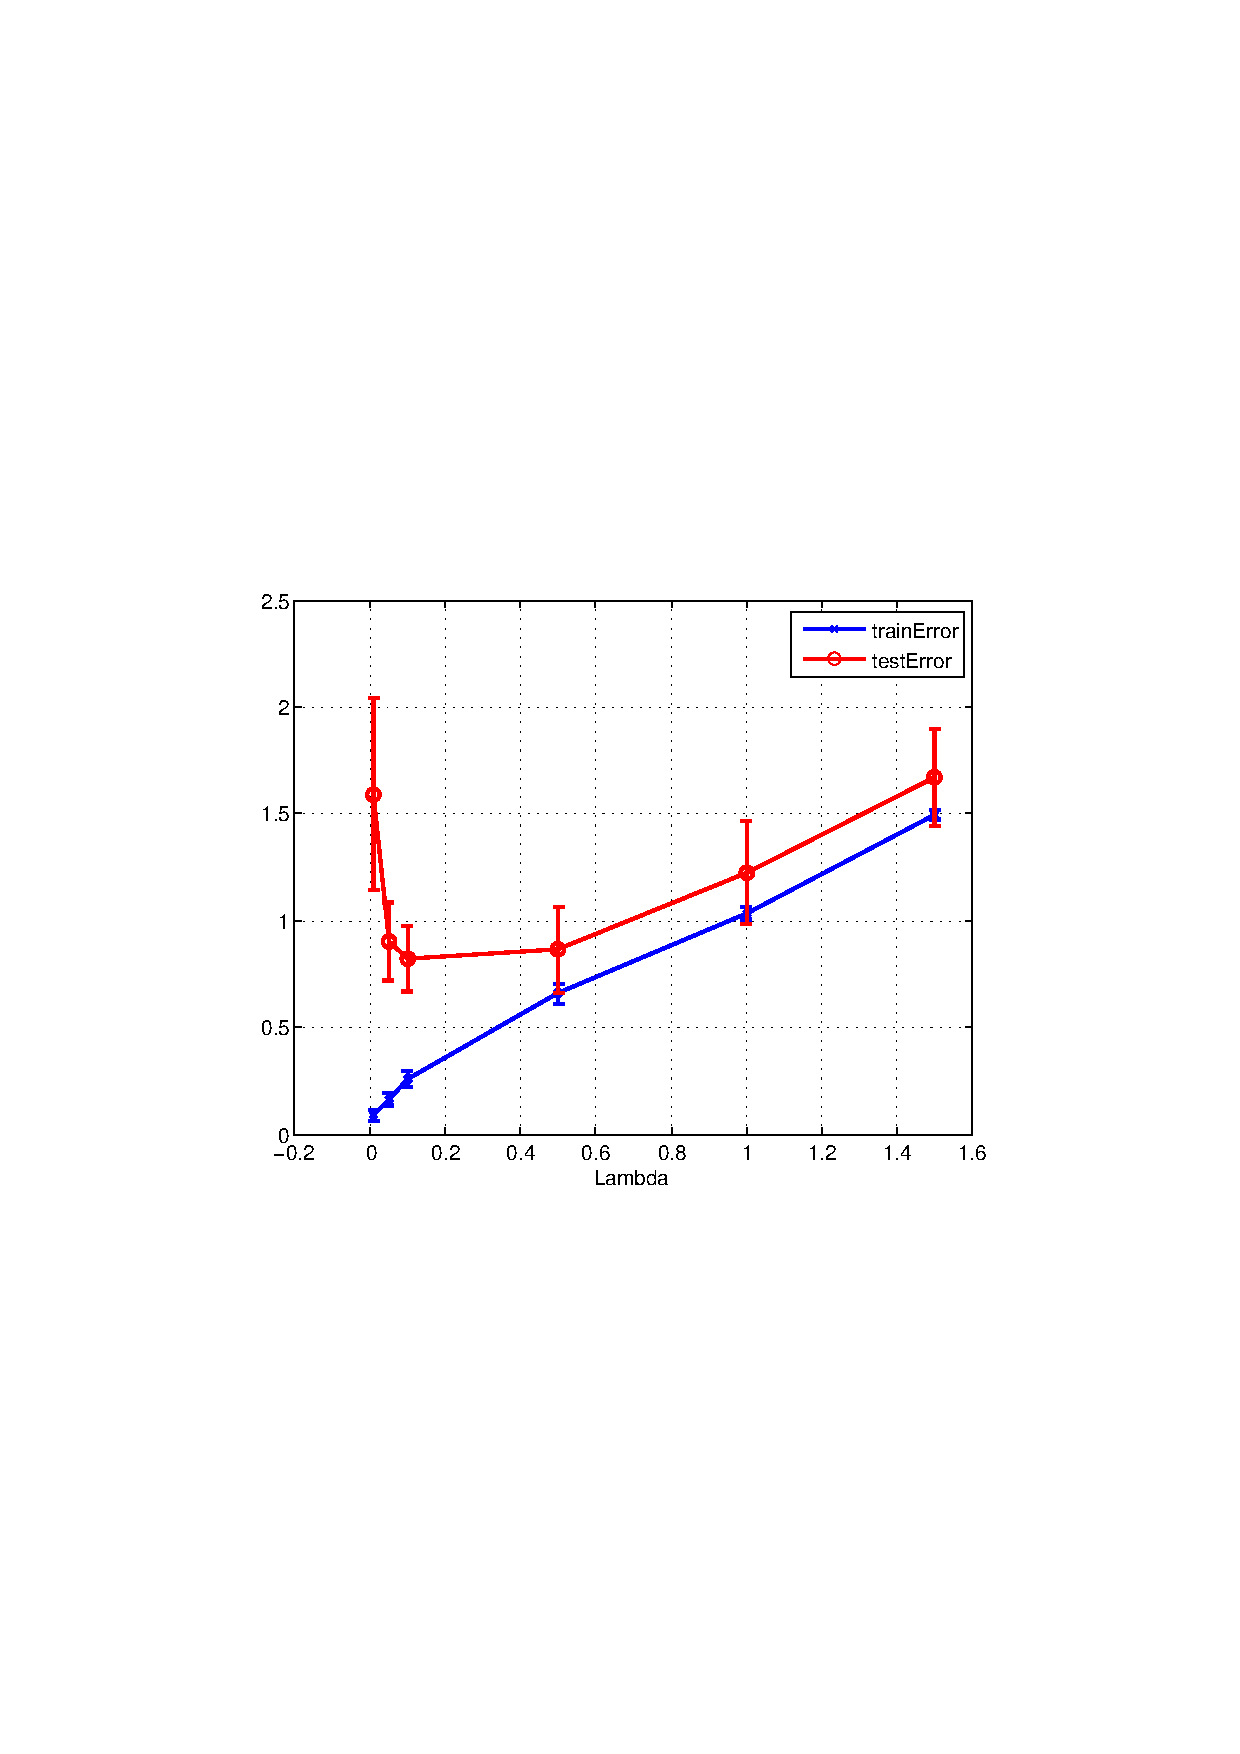
\includegraphics[clip, trim=4cm 9.2cm 3.5cm 9cm, width=\textwidth]{figures/ALS_lambda.pdf}
    %\captionof{figure}{Comparison of Train and Test errors with different lambda values}
    
  \end{minipage}
  \hfill
  \begin{minipage}[b]{0.5\textwidth}
  \begin{center}
  \begin{tabular}{ |l | c | c| }
    \hline
     lamb & MAE train & MAE test \\ \hline
     0.01   & 0.088 ($\pm$  0.0008) &  1.591 ($\pm$ 0.015) \\ \hline
     0.05  &  0.163 ($\pm$  895) &  0.901 ($\pm$  0.0061) \\ \hline
     0.1     & 0.259 ($\pm$ 851)  & 0.822 ($\pm$ 0.0012) \\ \hline
     0.5    & 0.660  ( $\pm$ 851) & 0.864 ($\pm$  0.0016)\\ \hline
     1       & 1.035 ($\pm$ 842) & 1.222($\pm$  0.0010)\\ \hline
     1.5    & 1.493 ($\pm$ 837) & 1.670($\pm$  0.0007) \\
    \hline
  \end{tabular}
  	%\label{table:labda_choice}
\end{center}
	\vspace{10 mm}
    \end{minipage}
    
\captionof{figure}{Estimated Train and Test MAE for different lambdas} 
\label{fig:ALS_lambdas} 
  \end{minipage}
\end{figure}  
  
%We notice that the test error across the 10 different splits of the cross validation has values from 2000 to up to 6000. This is an artifact of the high listening counts present in the long tail and the randomness of the split.
%\begin{figure}[h]
%  \centering
%  \begin{subfigure}[b]{0.45\textwidth}
%   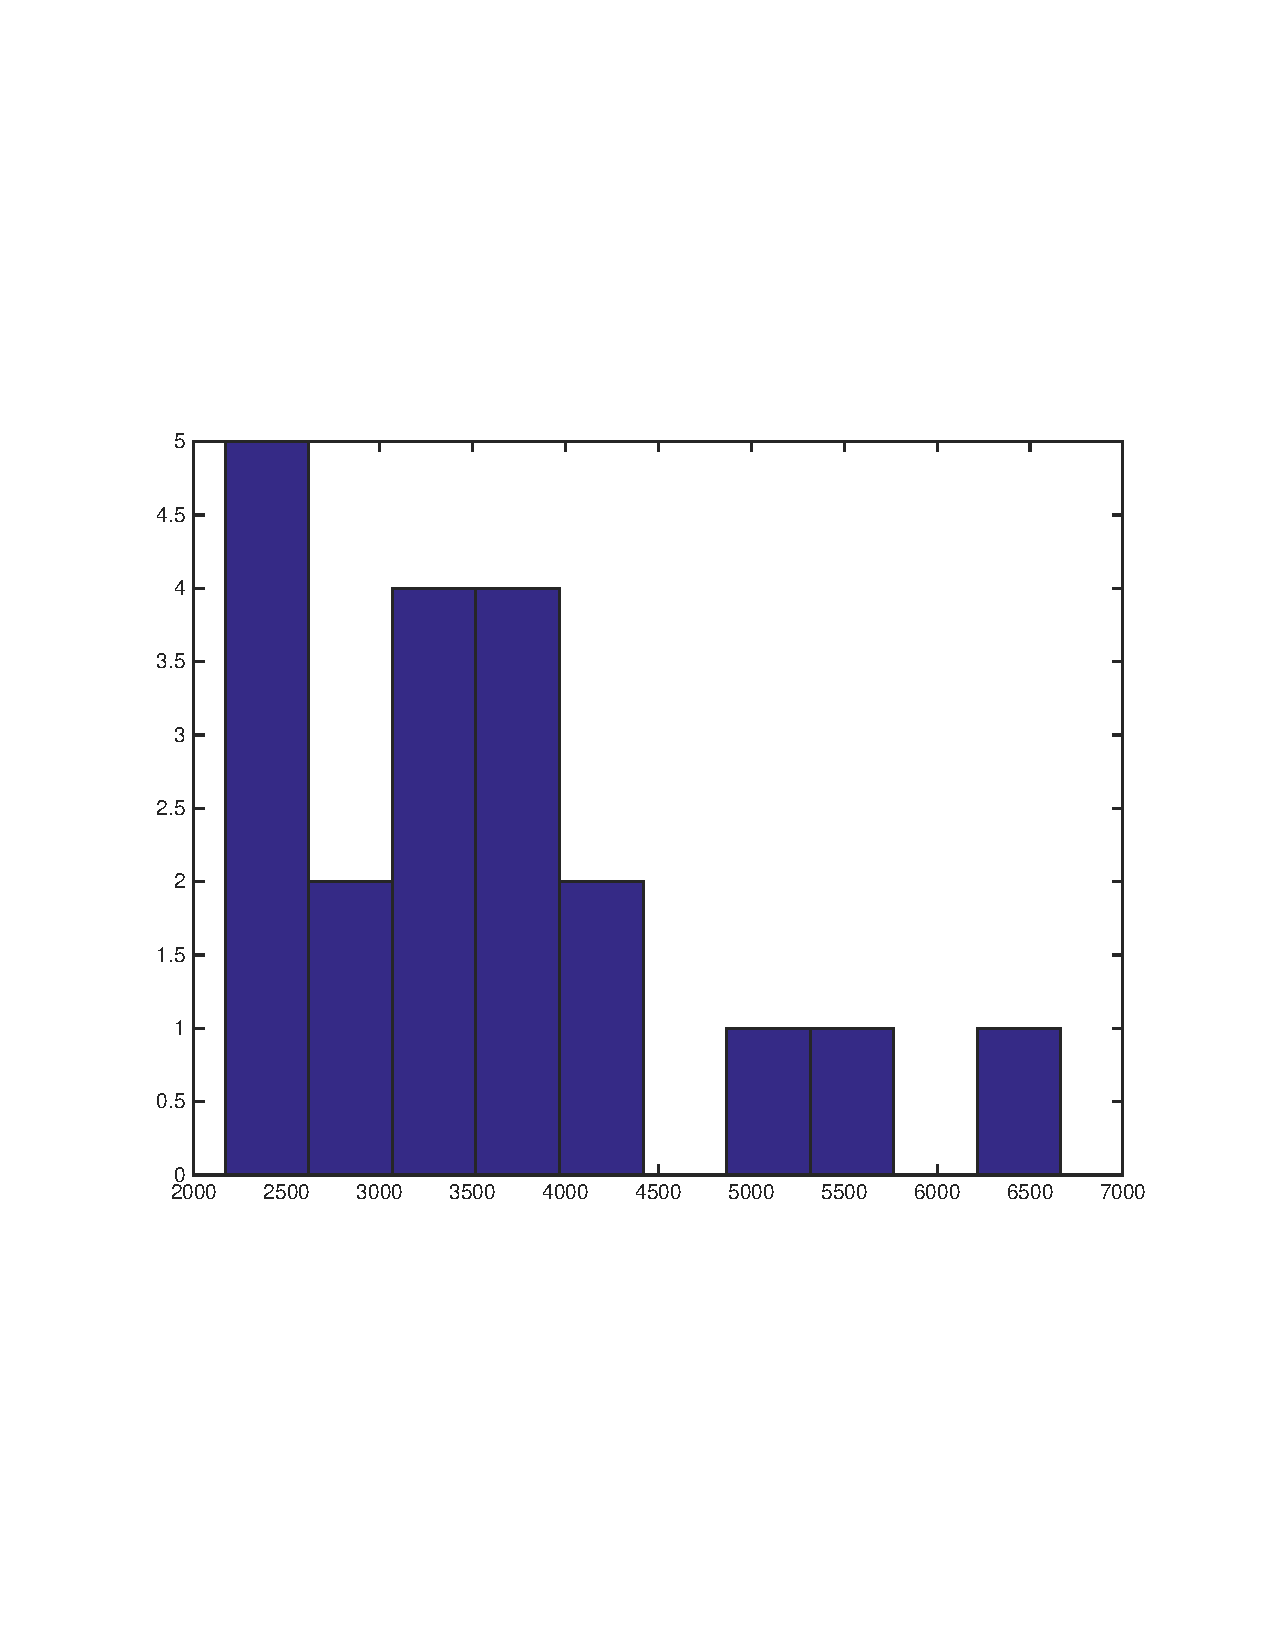
\includegraphics[width=\textwidth]{figures/distributionRMSE.pdf}
%    \caption{}
%  \end{subfigure}
%  \begin{subfigure}[b]{0.45\textwidth}
%    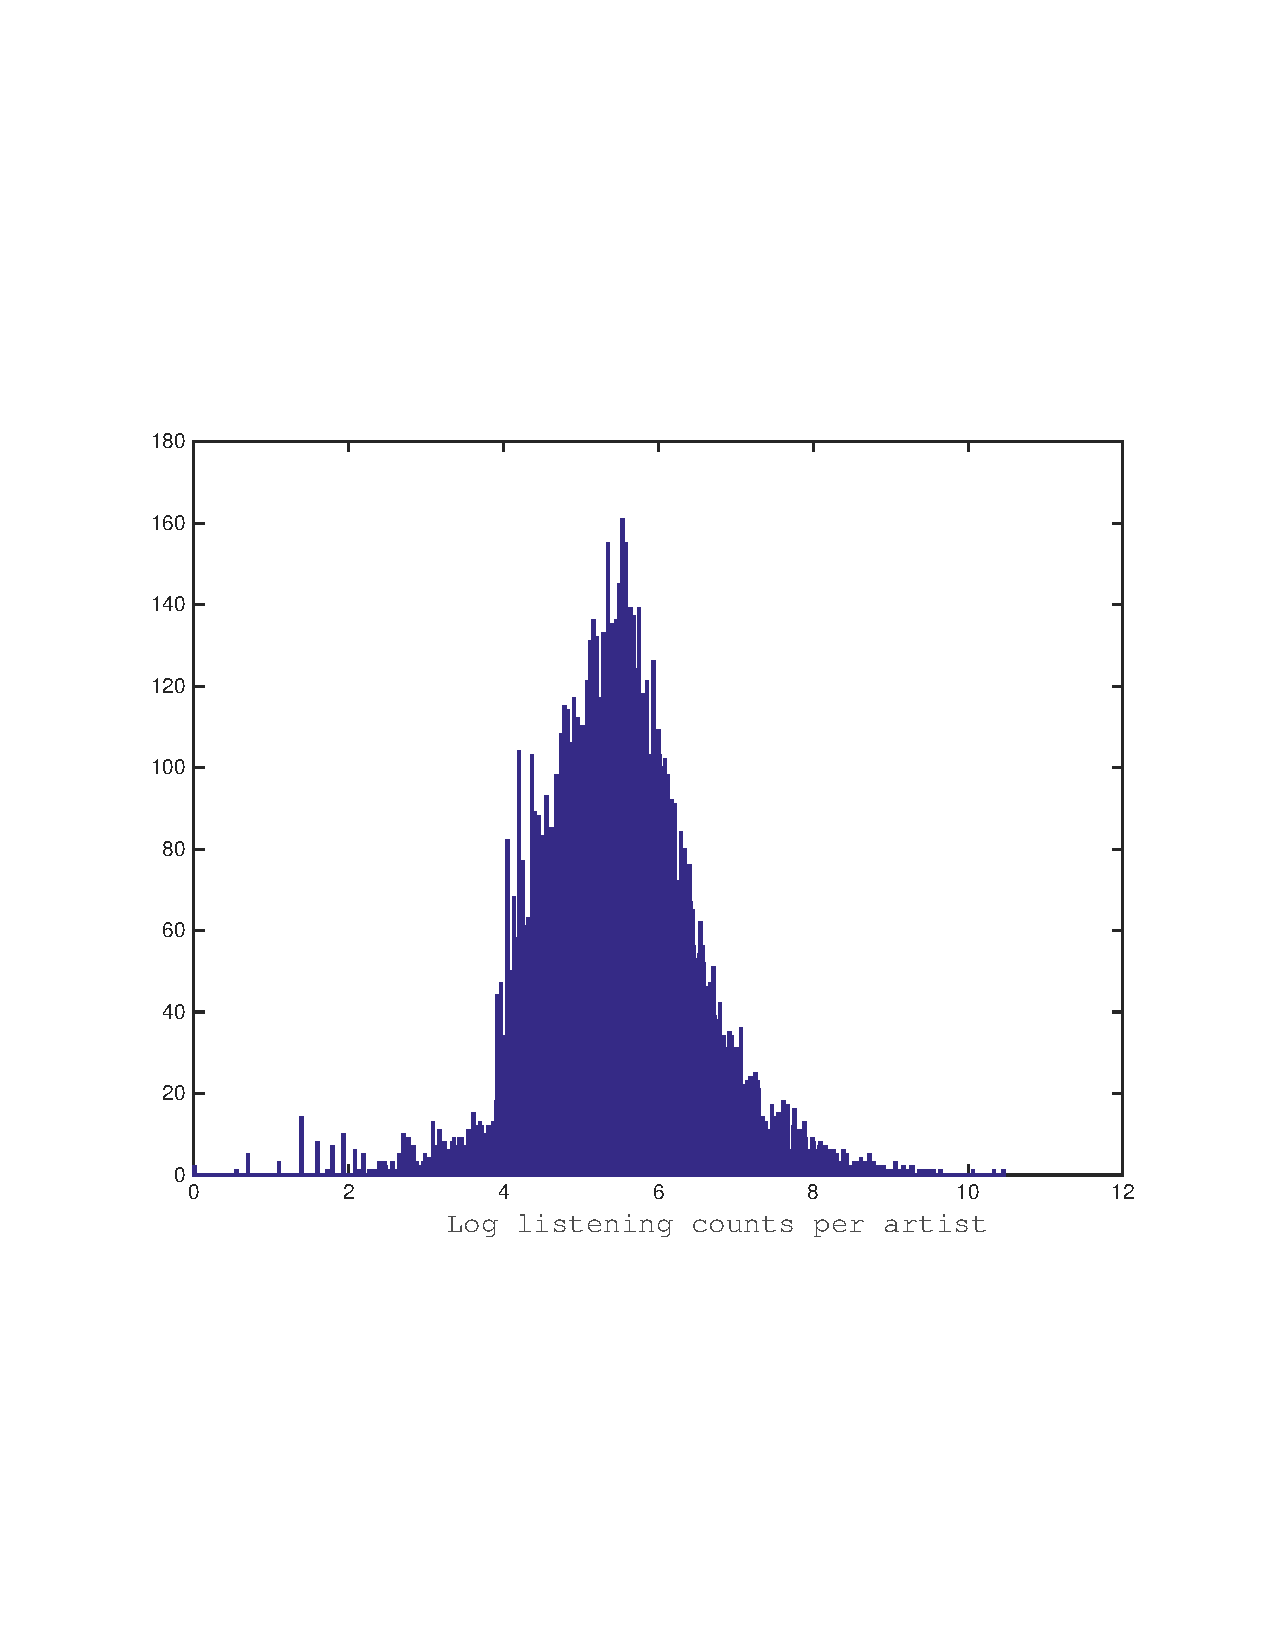
\includegraphics[width=\textwidth]{figures/histCountPerArtist.pdf}
%    \caption{}
%  \end{subfigure}
%  \caption{Distribution per user (a) and per artist(b) log of listenining count distribution}
%  \label{fig:new_plot}
%\end{figure}

\begin{figure}[h]
 \begin{minipage}{\textwidth}
  \begin{minipage}[b]{0.45\textwidth}
\centering
    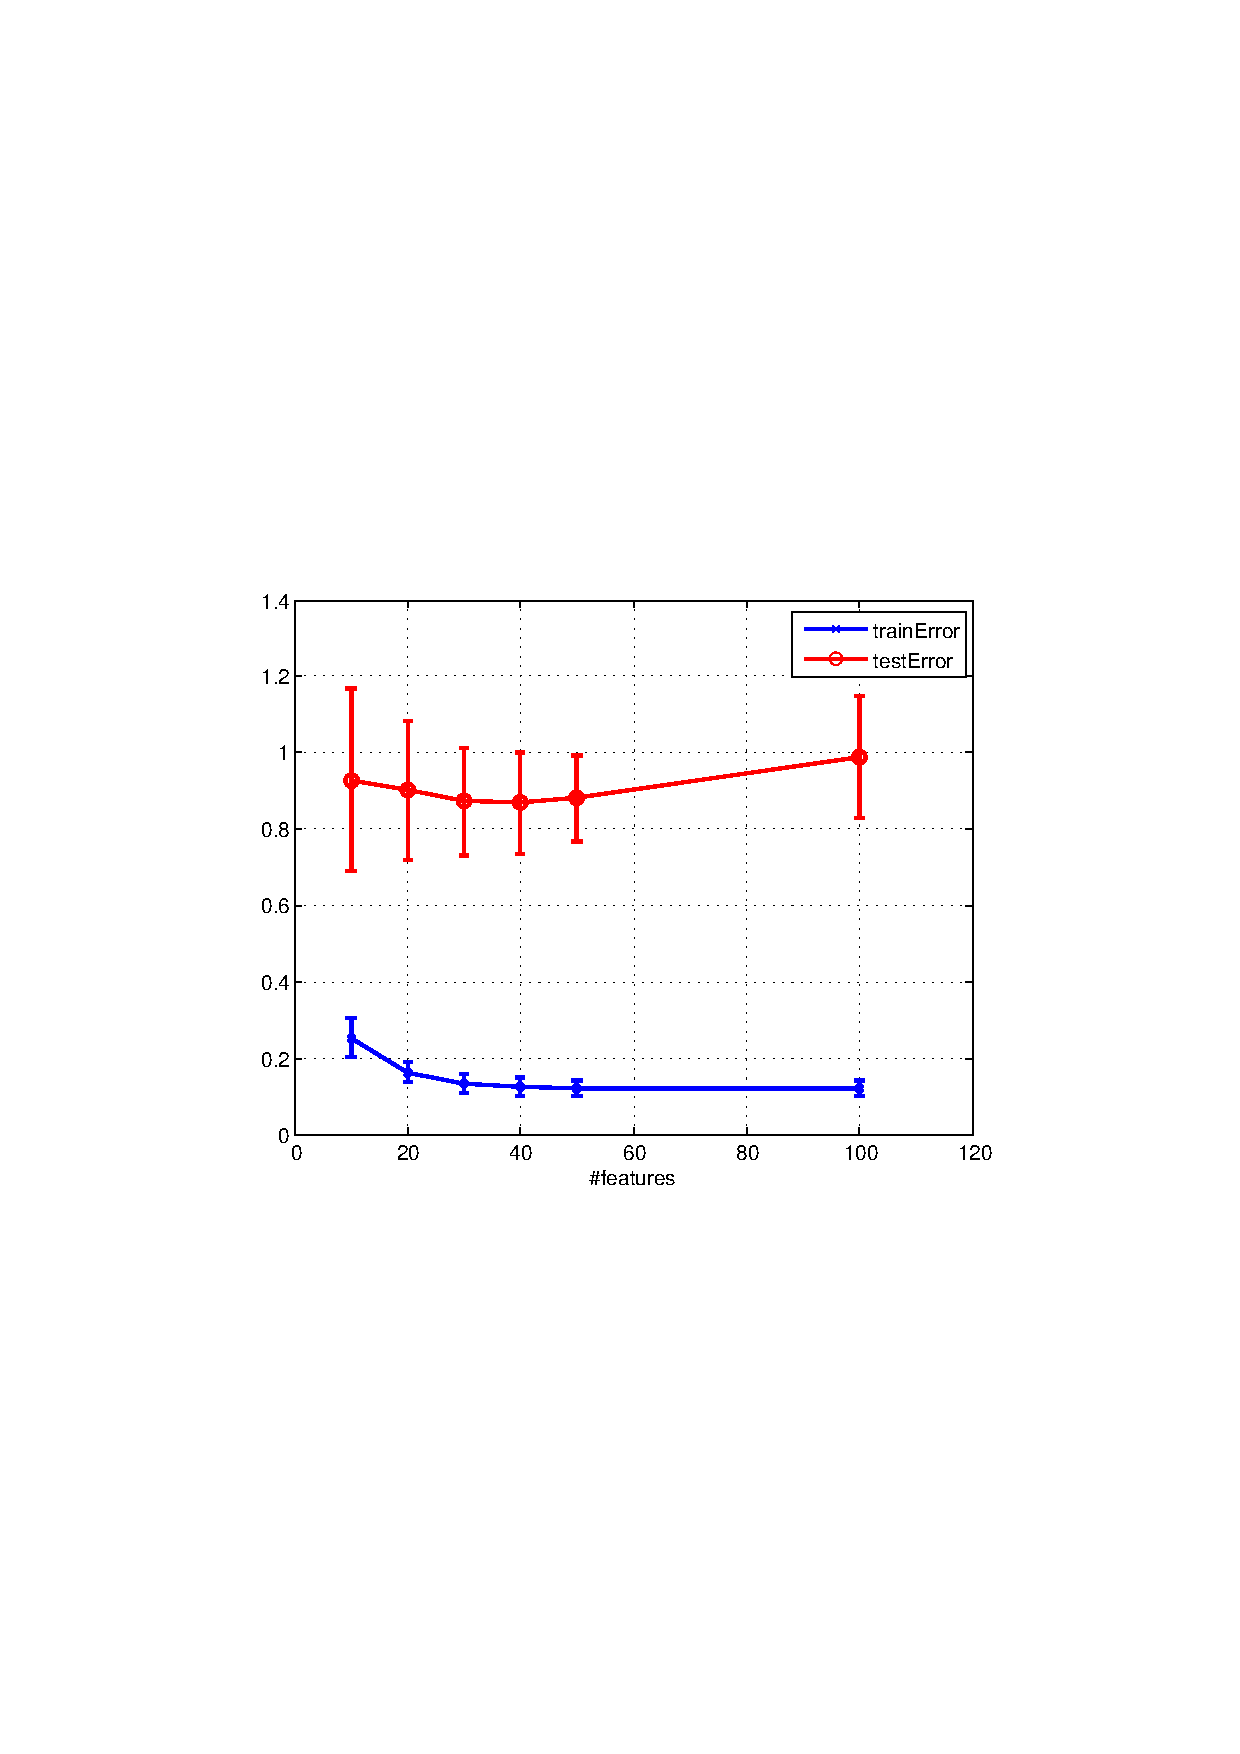
\includegraphics[clip, trim=4cm 9.2cm 3.5cm 9cm, width=\textwidth]{figures/ALS_features.pdf}
    %\captionof{figure}{Comparison of Train and Test errors with different features values}  
    
  \end{minipage}
  \hfill
  \begin{minipage}[b]{0.5\textwidth}
\begin{center}
  \begin{tabular}{ |l | c | c| }
    \hline
     feat & MAE train & MAE test \\ \hline
     10   & 0.253 ($\pm$  0.0017) &  0.927 ($\pm$ 0.0080) \\ \hline
     20  &  0.163 ($\pm$  0.0009) &  0.901 ($\pm$  0.0061) \\ \hline
     30     & 0.133 ($\pm$ 0.0009)  & 0.873 ($\pm$ 0.0047) \\ \hline
     40    & 0.124  ( $\pm$ 0.0008) & 0.868 ($\pm$  0.0044)\\ \hline
     50       & 0.121 ($\pm$ 0.0007) & 0.880($\pm$  0.0038)\\ \hline
     100    & 0.122 ($\pm$ 0.0007) & 0.989($\pm$  0.0053) \\
    \hline
  \end{tabular}
  	%\label{table:feature_choice}  
\end{center}
\vspace{10 mm}
    \end{minipage}
  \end{minipage}
  \caption{Estimated Train and Test MAE for different features}
  \label{fig:ALS_features}
\end{figure}
  
We varied the number of features from $10,20,30,40,50,100$ with $\lambda = 0.05$ (see Fig. \ref{fig:ALS_features}), and the train error increased from $0.122$ to $0.253$ while the test MAE reaches a maximum of $0.989$ and a minimum of $0.88$. Even though value $50$ for features is best for train error, we choosed $40$ because it gave slightly better results on the test set. The best setup gave a MAE less than $0.8$ for the test error when $\lambda=0.05$ and $40$ features.

%\begin{figure}[h]
%  \centering
%  \begin{subfigure}[b]{0.45\textwidth}
%   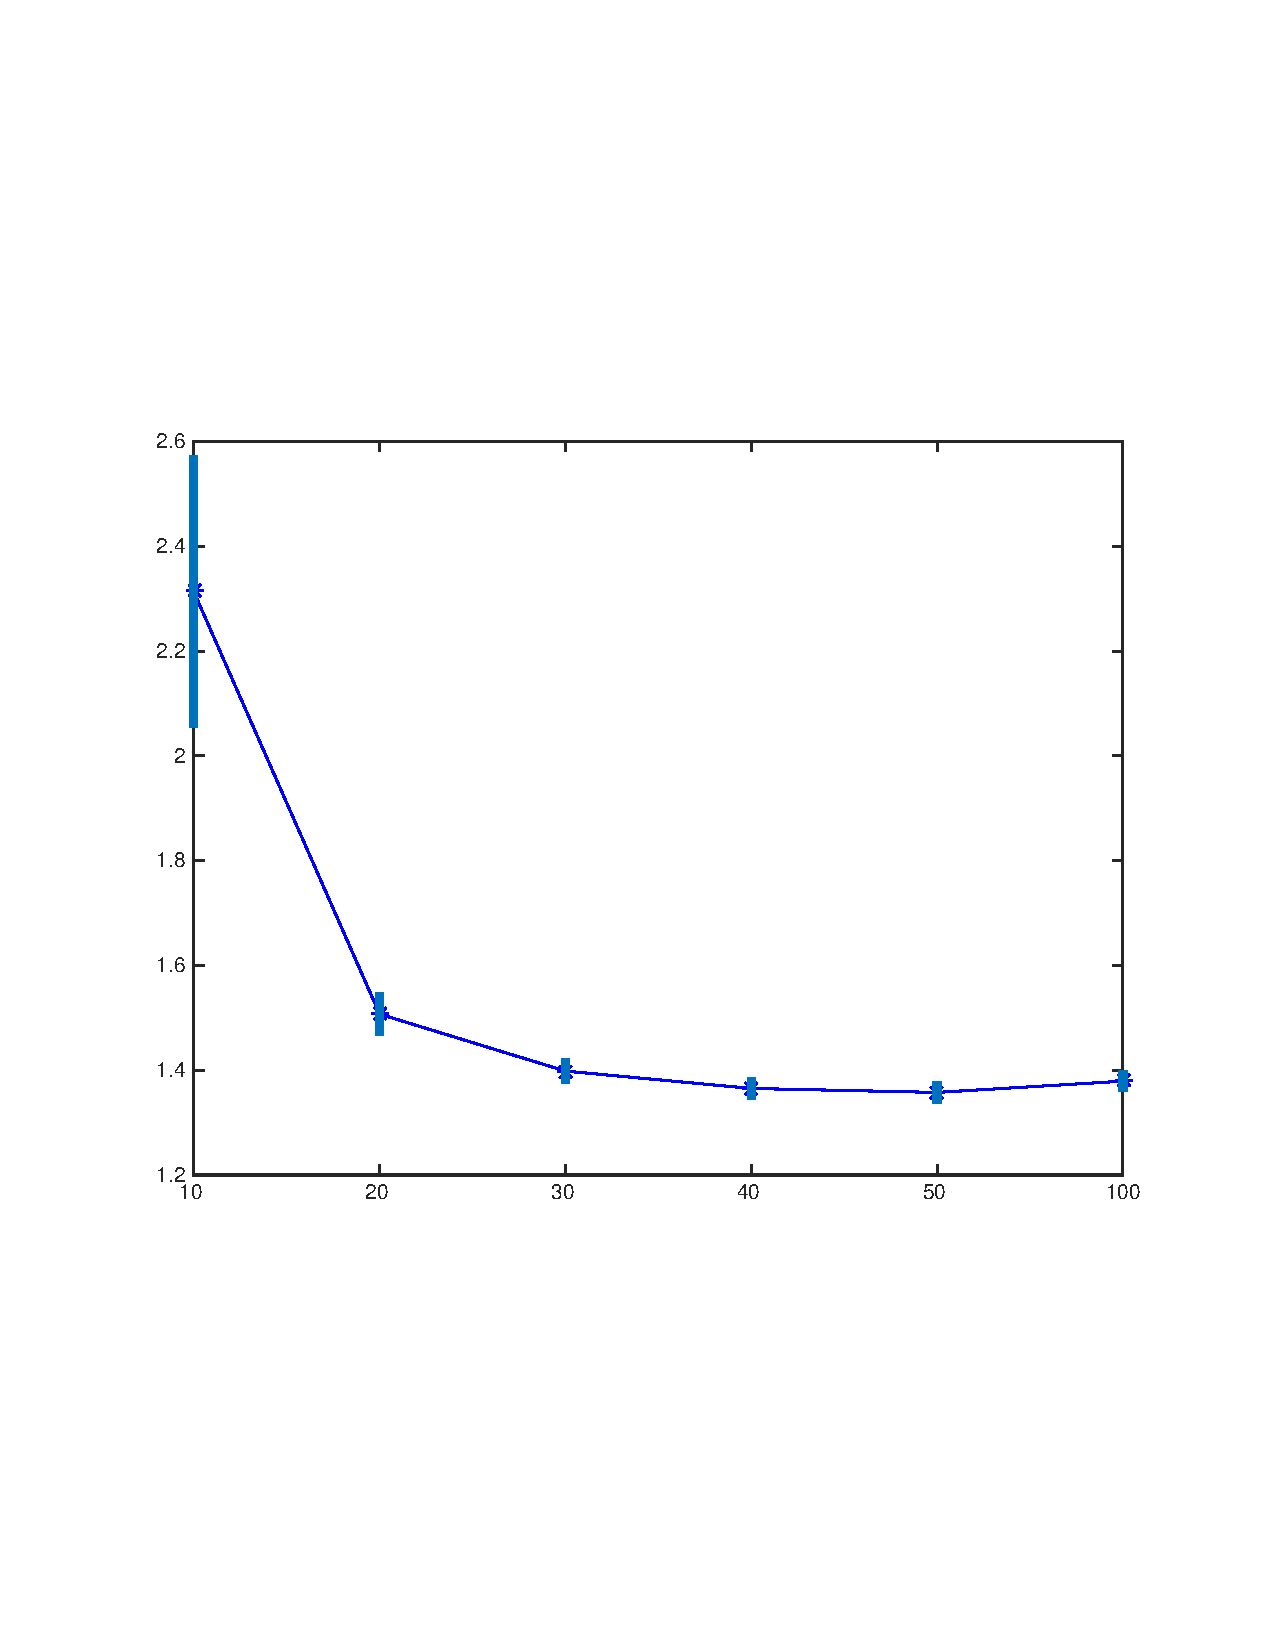
\includegraphics[width=\textwidth]{figures/als_train.pdf}
%    \caption{}
%  \end{subfigure}
%  \begin{subfigure}[b]{0.45\textwidth}
%    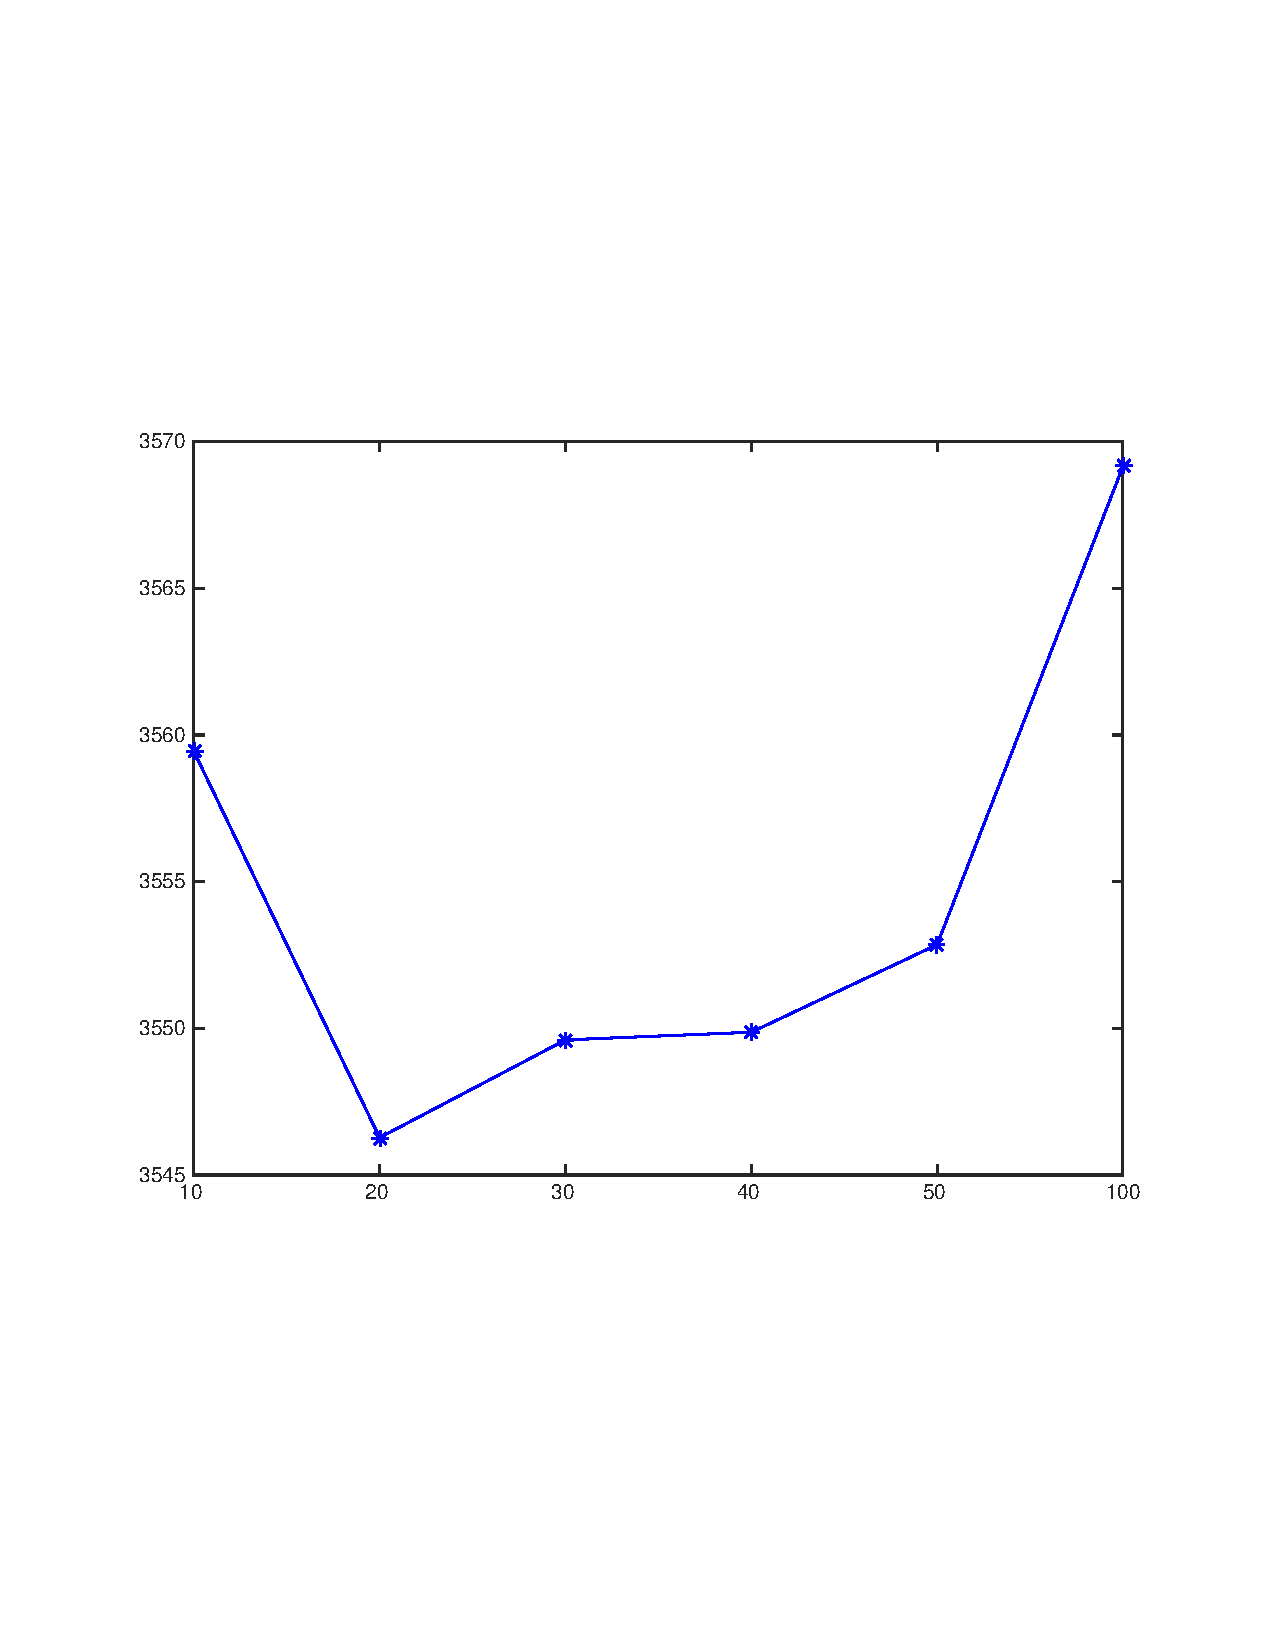
\includegraphics[width=\textwidth]{figures/als_test.pdf}
%    \caption{}
%  \end{subfigure}
%  \caption{Train and Test RMSE for logALS with varying number of features}
%  \label{fig:new_plot}
%\end{figure}

\subsubsection{K-means}
%Although the number of artists is 10 times larger than the number of users, 
For this model, we chose to implement K-means with clustering of users instead of artists so that we can use the clusters obtained here also in Task 2.

%, although that did not have a huge impact on our results.
The missing entries in the matrix were initialized with the user average. We then sorted the users according to their average score and initialized the clusters with equally spaced samples from the sorted users array. The goal of this cluster initialization was to have a more equilibrated assignment of users to clusters and to make sure we have clusters from both highly active and also from less active users.

Inspired by the friendship graph information, we tried K-means with varying number of clusters from [3,10,20,30,40,50,100]. We plot the mean train and test error using 10 fold cross validation in Fig \ref{fig:kmeans_final}. Using only 3 clusters both the train and the test error was high, while for 100 clusters the difference between train and test error became larger, giving signs of overfitting.

%We noticed also the fact that sometimes the training error of Kmeans (reported by taking exp of data and RMSE) had small fluctuations and it was not always decreasig as the algorithm convergence properties would expect. This is due to the fact that Kmeans miminizes squared error but our cost is a little different since we transform the data using exp.

%\textcolor{red}{change figure 6b with plot user mean count and variance.}
%\textcolor{red}{Add comparison.}

\begin{figure}[h]
  \centering
  \begin{minipage}[b]{0.42\textwidth}
   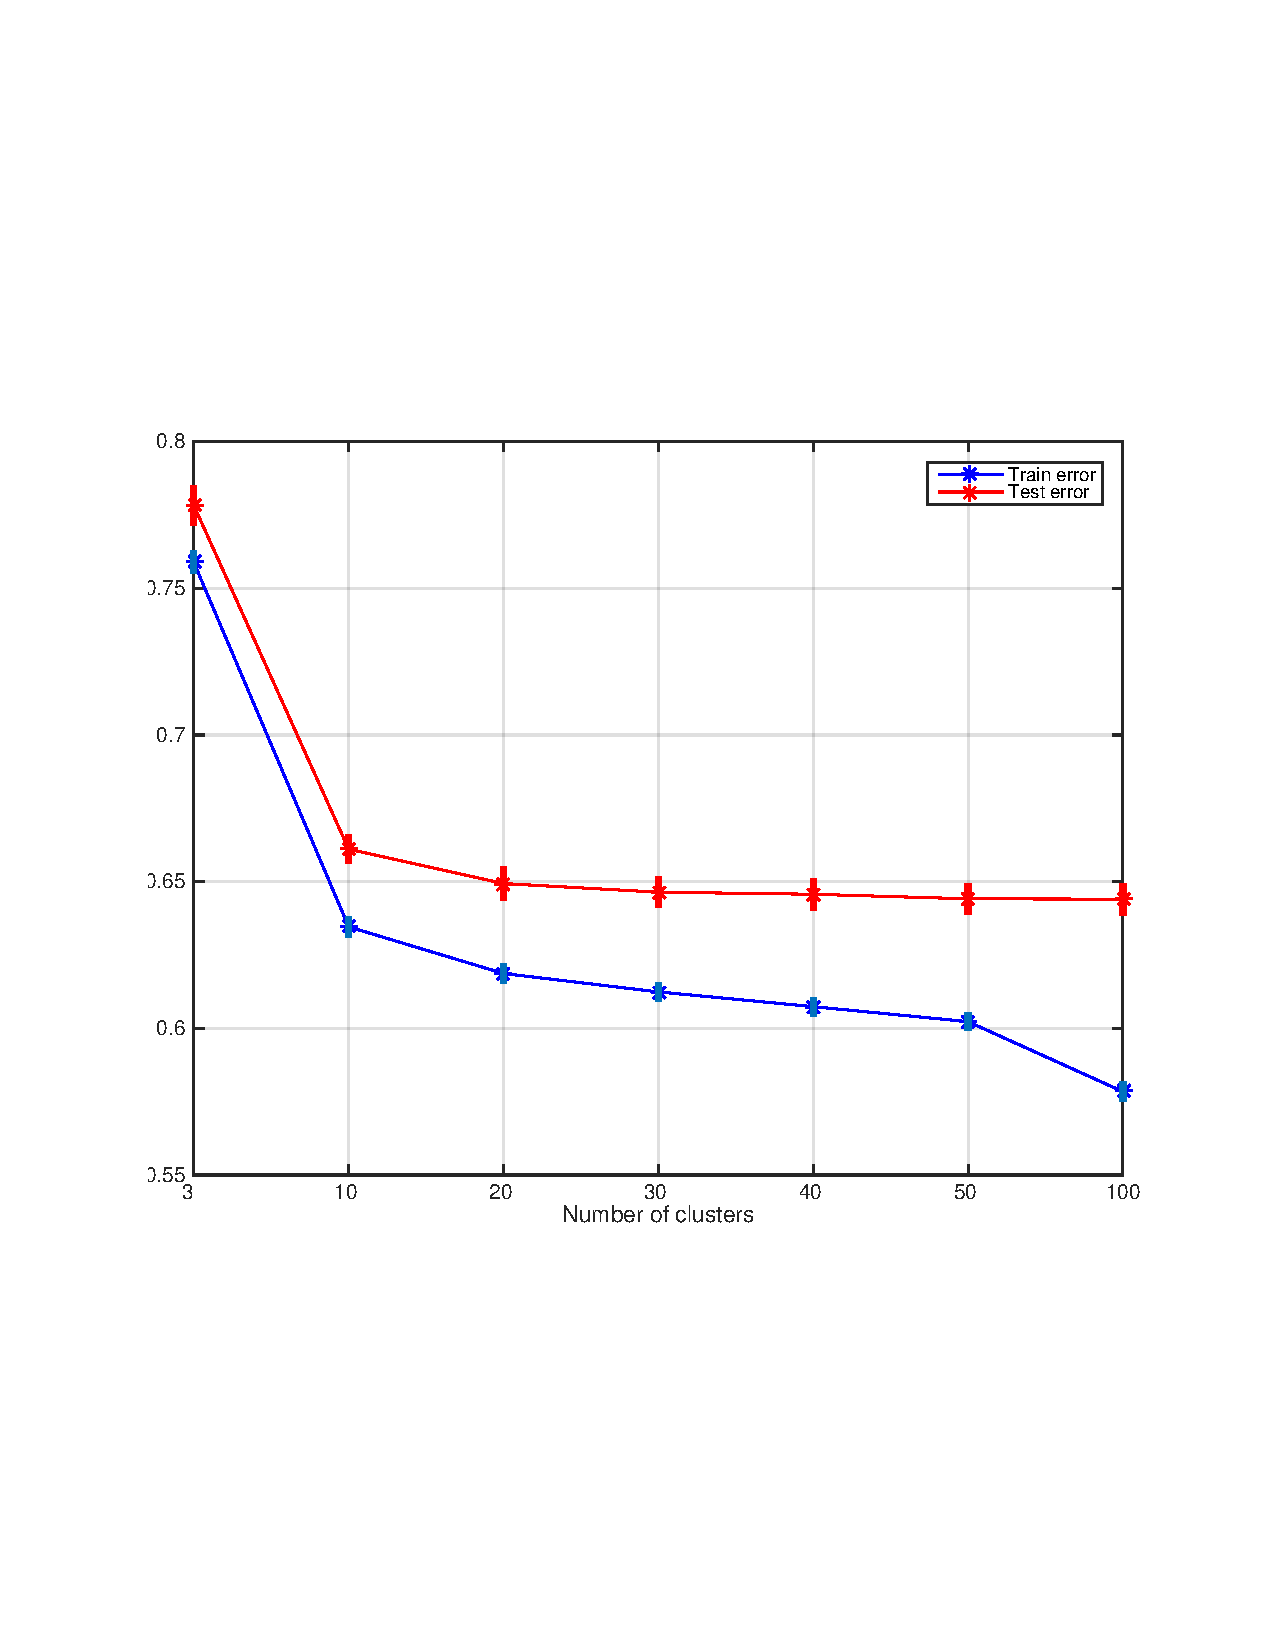
\includegraphics[width=\textwidth]{figures/kmeans_train_test.pdf}
    \caption{Estimated Train and Test MAE for different cluster counts}
    \label{fig:kmeans_final}
  \end{minipage}
  \hfill
  \begin{minipage}[b]{0.45\textwidth}
    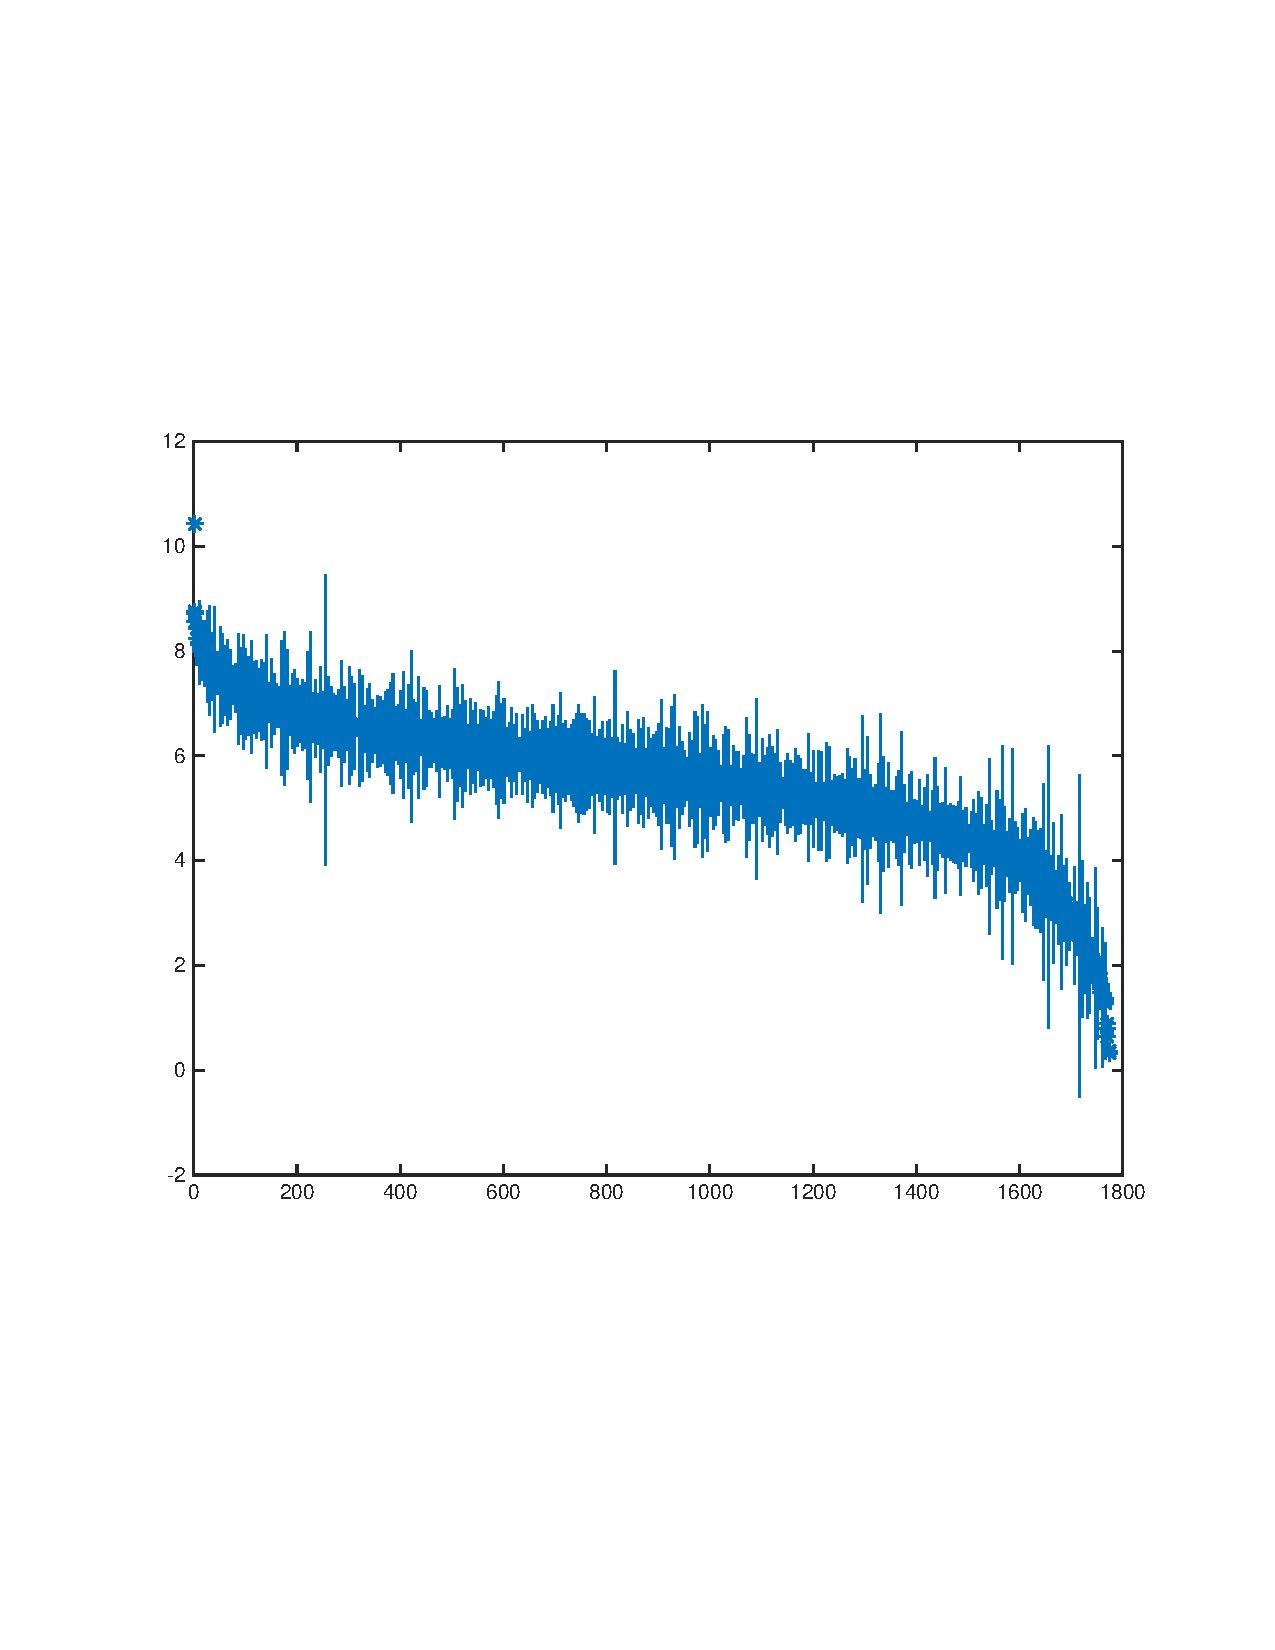
\includegraphics[clip, trim=2cm 6.8cm 1.5cm 7cm, width=\textwidth]{figures/MeanStdCountPerUser.pdf}
    \caption{Average count per user}
    \label{fig:MeanStdCountPerUser}
    \vspace{2 mm}
  \end{minipage}
  %\caption{bla bla}
\end{figure}

In all the experiments with more than 20 clusters we obtained a test MAE close to 0.64. This was our best test MAE so far. For computational reasons, we picked 20 clusters for the next task.

%We also tried K-Means in the update step, only the entries for artists that were known were updated. We expected this to perform better, but the algorithm had problems with overfitting, always giving a train error less than 0.4 (much less than the normal Kmeans) but a test error a bit over 0.7 (higher than the normal KMeans). This happened for all the cluster sizes we experimented with.

\subsection{Comparison}

KNN algorithm (MAE $1.49$) is unsuccessful compared to other methods, even worst than baseline global average. The possible reasons are the high sparsity of our data and the choice of the similarity measure. It is known that KNN has limitations in performing well on sparse data matrices. Even though ALS method (MAE $0.8$) gave better results, it still didn't perform better than user mean baseline method and k-means. The K-means algorithm (MAE $0.64$) is similar to the expectation-maximization algorithm for mixtures of Gaussians meaning that they both attempt to find the centers of natural clusters in the data. Our results show that Kmeans appears to be a suitable approach for our problem, but we believe that its good performance comes from the sparsity-reduction step where we initialize the missing values. Both Kmeans and user mean average baseline perform well because they incorporate good estimates on the missing entries.

\subsection{Task 2}
In this task we make predictions for a set of new users using their friendship information with a set of old users for which partial listening history is available. In other words, we try to see if there is a correlation between
users' friendship and users' preference in music.

\subsubsection{Friendship information}
The initial friendship graph $Gtrain$ of $1776$ nodes and $22904$ edges contained $22$ connected components, but the majority of the components contained just a few nodes.
Using the Gephi  \footnote{http://gephi.github.io/} tool we were able to find some properties of the graph such as the number of communities, 32 (out of these, only 8  had more than 150 members).
These statistics were run so that we get an idea of the number of friendship clusters present. The number of connected components and of communities are similar with our choice of 20-30 clusters in KMeans .

We have tried two approaches using the friendship information, one based on the mean average per user and one based on Kmeans clustering of users.

\subsubsection{Baseline Methods}
As a reference method, we predict for a missing value the global average of all the available counts, which gave us a MAE of 1.078($\pm$0,044). Taking the average per artist gave us a MAE of 1.767($\pm$  0.09), significantly worse than the one above.

\subsection{Mean of Friends Method}
In this approach, a prediction for a new user $Ystrong(u,a)$ is computed as the average count of its friends' listening counts $Ytrain(f,a)$ for that artist or global average count for an user without friends.

\begin{table}[h]
  \centering
  \begin{tabular}{ c  l }
  $Ystrong(u,a) $&= $\frac{\sum_{f\in Friends(u), Ytrain(f,a)\neq0}{Ytrain(f,a)}}{n\_fa}, n\_fa \neq 0$ \\ 
                          &= $global\_average, n\_fa = 0$ \\ 
  \end{tabular}
\end{table}
where $n\_fa$ is the cardinality of the set $\left\{ Ytrain(f,a)\neq0, f\in Friends(u)\right\}$

For this setup  we obtained a test MAE=1.52 ($\pm$0.29) which is smaller than our global average baseline prediction.
If we also take into account the friends of the friends of user $u$ we obtain  a MAE of 1.08($\pm$ 0.041). This result is comparable with our best baseline solution.

\subsubsection{KMeans}
We clustered the users into 20 groups using the KMeans setup from Task 1
and repeated the experiments. For a new user,  we predict the count as the mean of its friends and its friends' friends clusters. This gave us a MAE of 1.08($\pm$ 0.04). This is similar with the best prediction from the previous approach and with the  global average baseline. Although KMeans with 20 clusters does not seem to outperform the other methods, we decided to use this on our newly predicted data. Increasing the number of clusters did not seem to help, as we obtained the same performance with 30 clusters and worse results with 100 clusters (test MAE = 1.55). 
 
%We mention that we had other unsuccessful experiments where the prediction was done using the mean of the unique friends'clusters or using only the most frequent cluster among friends (test MAE = 1.49).

\subsection{Conclusions}
Our proposed methods did not outperform the global average prediction, giving comparable performance. These results are not conclusive enough to say if friendship information is indeed correlated with users' music listening counts (we believe it is). As further steps, we could analyze the correlation of the friendship information of the old users with their listening history. Basically, we could try to predict weak entries using only friendship information, information which we actually did not use in Task 1. Another helpful analysis is to see a histogram of the individual errors and the characteristics of the users for which friendship information is not useful.
